\chapter{Setting Up Eclipse}
\label{ch:Eclipse}

\section{Configuring Eclipse on the UCT Computers}
\label{sec:EclipseConfig}
Eclipse is fully configured on the UCT campus computers but there are some steps that you need to remember before getting started. First plug in your STM32 board, Windows should start searching for a pre-configured driver once it's plugged in.
\includegraphics[height=3ex]{driverico}\\
\begin{figure}[htbp]
\centering
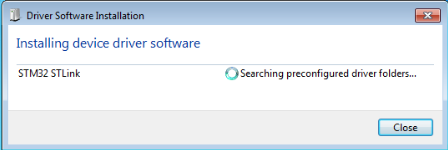
\includegraphics[width=0.6\textwidth]{driverinst}
\end{figure}
\\
Windows should eventually find the drivers and you're ready to go. Launch up Eclipse, it is important you leave the default workspace as \textbf{\color{Aquamarine}{C\textbackslash :Workspace}}.
\begin{figure}[htbp]
\centering
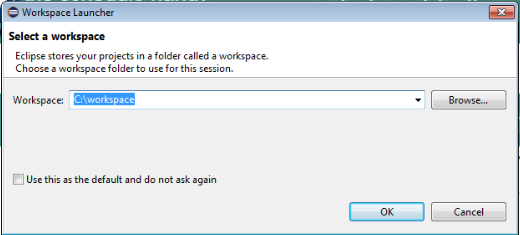
\includegraphics[width=0.8\textwidth]{workspace}
\end{figure}
\\
Then wait for \textbf{Eclipse} to load up, then create a new \textbf{\color{Green}STM32F0xx C\textbackslash C++ Project}. The compiler will load up all the relevant files and put out a pretty empty generic template. First off, build the project so you have a set of binaries (.ELF files) to work with. You Build a project by following $\textbf{Project}\rightarrow \textbf{Build All}$ ,or selecting \textbf{Build Project} by right-clicking on the project file in the File Explorer window.
\\
To run the code on your STM32 board, simply debug the project using the\textit{GDB OpenOCD Debugging} configurations. The UCT computers will auto detect the project you are working on (only if you've already built it). Conveniently, the config for OpenOCD is filled in already so you can debug your code from the \textbf{\color{Purple}Debug Perspective}.
\section{Configuring Eclipse for the STM32}
\label{sec:eclipseconfig}
The following is a guide to setting up Eclipse for Windows to debug the STM32F051 UCT Development board; I understand it is quite lengthy but it covers many details that are important when developing for the STM32. If your Eclipse is already set up, skip ahead to Perspectives in Eclipse \cite{sec:perpectives} to see how to navigate around the Eclipse environment.
\\
After installing Eclipse there is a section explaining Eclipses functionality and how to get the most out of your STM32 development board. Some of the installation steps may have already been completed in preparation for STM32 development in your previous courses, just skip those installations if they have already been performed on the computer you are setting up.
\subsection{Installation}
\label{subsec:inst}
\subsubsection{gcc-arm-none-eabi}
As with regular assembly development for the STM32F051 (hence forth the STM32), the standard arm development tools are needed to assemble our written source code (main.s) into an Assembly coded object file (main.o) and finally to link that object file to the particular memory addresses of our target processor (main.elf). 
So download and install the \textbf{GCC-ARM-NONE-EABI toolset} from {\color{Blue}\underline{\smash{\href{https://vula.uct.ac.za/x/m9Z91P}{Vula}}}}.Otherwise get it from the  {\color{Blue}\underline{\smash{\href{https://launchpad.net/gcc-arm-embedded}{official site}}}}\footnote{https://launchpad.net/gcc-arm-embedded}.
\\
Remember that this is a 32-bit version of the development tools consisting of 32-bit executables. Even if you are running a 64-bit system you will still be using these tools. Once the files are extracted you will be prompted to \textbf{\color{Purple}"Add path to environment variable"}
\begin{figure}[hbtp]
\centering
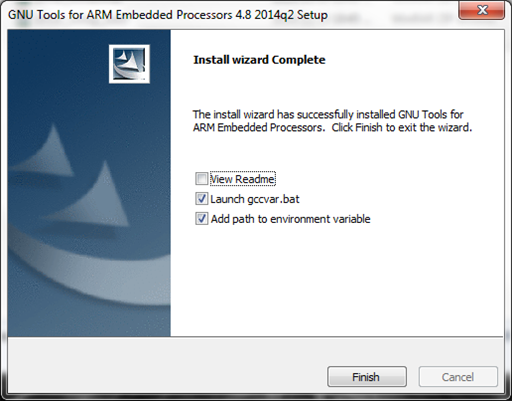
\includegraphics[width=0.6\textwidth]{gccinst}
\end{figure}
\newpage
You'll want to select this parameter, it adds the location of all the .exe's to your Windows advanced system settings so they can be run from any location without having to navigate to \textbf{\color{Aquamarine} C:\textbackslash Program Files (x86)\textbackslash Gnu Tools Arm Embedded\textbackslash ... }
\\
You don't need to worry about the Readme or GCCVAR.bat, so deselect both and finish the installation. Included in the GNU Tools we've just installed are debugging, compiling and linker tools provided specifically for Arm development, its' an open source tool chain which you can read about on the official GCC-Arm-Embedded website. Just to ensure that it is installed correctly (and the system path has been added to your environment variable correctly), from your command line run;
\\
\-\ \hspace{20pt} \textbf{\color{YellowGreen} \$  arm-none-eabi-as --version}
\\
It should produce some details about the current GNU assembler version (this test is applicable for any of the GCC Arm tools; \textbf{ls}, \textbf{gdb} etc \ldots)
\begin{figure}[hbtp]
\centering
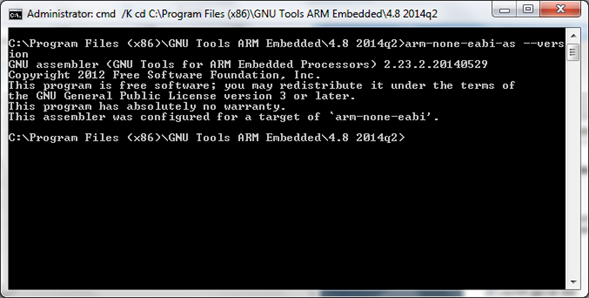
\includegraphics[width=0.6\textwidth]{gccinfo}
\end{figure}
\\
A useful trick to note is that, within any file in windows, pressing the SHIFT key and right clicking inside the folder gives you the ability to open a command window (CMD) at the files current location. This isn't really important but it might come in handy.
\begin{figure}[hbtp]
\centering
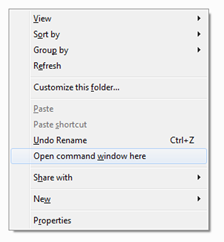
\includegraphics{cmdwindow}
\end{figure}
\newpage
{
\color{Red} \underline{\smash{If you receive an error}} in which the command is unrecognized it means you either have not installed the tools correctly or the environment variable path has not been appended.
\begin{figure}[htbp]
\centering
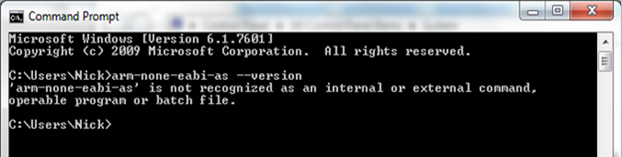
\includegraphics[width=0.9\textwidth]{armerror}
\end{figure}
\\
To add the path variable you must navigate to:
\\
\centering
\textbf{\color{Green} Control Panel $\rightarrow$ Advanced System Settings $\rightarrow$ Environment Variables}
\\
\begin{figure}[hbtp]
\centering
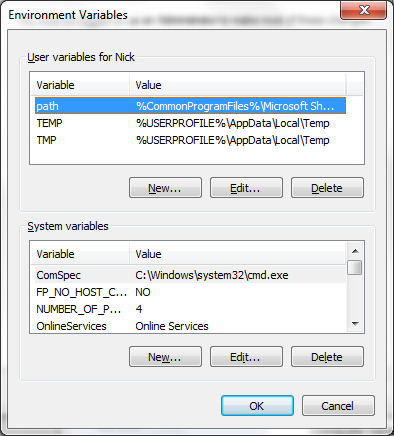
\includegraphics[width=0.6\textwidth]{envvar}
\end{figure}
\raggedright
We want to edit the \textbf{path variable} , in the variable value paste (the semi-colon is VERY IMPORTANT):
\\
\centering
\textbf{\color{Aquamarine} C:\textbackslash Program Files (x86)\textbackslash GNU Tools ARM Embedded\textbackslash 4.8 2014q2\textbackslash bin;}
\\
\raggedright
and then accept this by pressing OK until you are out of the system properties tab. Depending on where you installed your Tool Chain to be, this location may change so find the \textbf{bin} folder within that location and add that value to the path variable
}
\newpage
\subsubsection{Install OpenOCD}
Next we need to install OpenOCD, the on chip debugging utility that lets us upload our code onto our target STM32. The debugging process takes place between the ST-Link device and the target STM32. What you may not realize is that the ST-Link is actually another specially programmed STM32 microcontroller. The  ST-Link receives code from the computer, pretty much line by line, it then prepares our target STM32 to receive new code to be flashed to its memory by pulling some pins high/low in a particular order and finally it feeds our code to the target micro via a communication standard called JTAG.
\\
Download {\color{Blue}\underline{\smash{\href{https://vula.uct.ac.za/x/sRNwF6}{OpenOCD-0.8.0.zip}}}} from Vula or {\color{Blue}\underline{\smash{\href{http://openocd.org/}{the OpenOCD Website}}}}\footnote{http://openocd.org/} and extract its' contents somewhere useful like in \textbf{\color{Aquamarine} C:\textbackslash Program Files\textbackslash OpenOCD}
\par
\emph{\color{Gray} Remember the location (file name) to which you extracted OpenOCD to, mine is called OpenOCD and is in the location listed above, and yours might be different.}
\par
Then navigate to \textbf{\color{Aquamarine}C:\textbackslash Program Files\textbackslash OpenOCD\textbackslash bin-x64} and then rename executables:
\\
\textbf{\color{Orange}openocd-x64-0.8.0.exe} to \textbf{\color{Orange}openocd.exe}
\\
This just makes things a bit easier for us. We now want to add OpenOCD’s path to the Environment Variables so once again, navigate to:\\
\textbf{\color{Green} Control Panel $\rightarrow$ System $\rightarrow$ Advanced System Settings $\rightarrow$ Environment Variables\ldots}
\\
Editing the path variable, we will see there is already a value for arm-none-eabi’s tools which was added in Step 1, so after this we \underline{\smash{append}} or paste in the location of OpenOCD:
\\
\underline{\smash{(NOTE: the semi-colon is VERY IMPORTANT)}}
\\
\textbf{\color{Aquamarine} C:\textbackslash Program Files\textbackslash OpenOCD\textbackslash bin-x64\textbackslash openocd.exe;}
\par
\fbox{
\begin{minipage}[c]{0.9\textwidth}
\color{Red}
Make sure there are \underline{\smash{no spaces}} between each subsequent path variable, only semi-colons. Mine looks like:
\\
{\raggedright \textbf{C:\textbackslash ~MinGW\textbackslash bin;C:\textbackslash ~Program Files ~(x86)\textbackslash ~GNU Tools ~ARM Embedded\textbackslash ~Q2\textbackslash ~bin;C:\textbackslash ~Program ~Files\textbackslash ~OpenOCD\textbackslash ~bin-x64;}}
\\
If there are spaces after the semi-colons, windows won't recognize the paths as system variables and it won't work!
\end{minipage}
}
\par
Finally, test the path has been added correctly by running the following in the command line:\\
\-\ \hspace{20pt} \textbf{\color{YellowGreen} \$ openocd.exe --version}
\\
And you should be rewarded with some more version details\ldots
\\
\begin{figure}[hbtp]
\centering
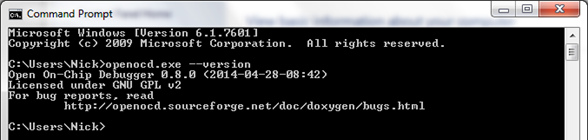
\includegraphics[width=0.7\textwidth]{openocdver}
\end{figure}
\newpage
\subsubsection{Install ST-Link Utility}
As mentioned above, the on chip debugger makes use of the ST-Link device (we use the ST-Link V2 in particular) so we obviously need some drivers and programs for all this to work. 
Download the {\color{Blue}\underline{\smash{\href{https://vula.uct.ac.za/x/8LNN3V}{ST-LINK Utility}}}} from Vula or {\color{Blue}\underline{\smash{\href{http://www.st.com/content/st_com/en/products/embedded-software/development-tool-software/stsw-link004.html}{ST Electronics' Site}}}}\footnote{$http://www.st.com/content/st_com/en/products/embedded-software/development-tool-software/stsw-link004.html$} and install the utility. This will also install the ST-Link USB drivers as well as the device utility (choose to \textbf{\color{Purple} Trust/Install} the STMicroelectronics Ports (COM \& LPT) device software)
\\
\begin{figure}[htbp]
\centering
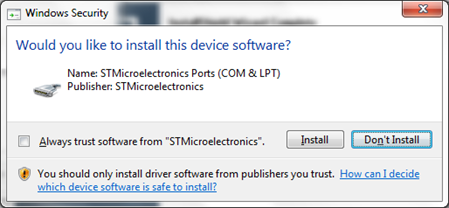
\includegraphics[width=0.6\textwidth]{installstutil}
\end{figure}
\\
For some reason the installation attempts to install the device drivers twice, just click \textbf{Next} and it will take you through to the end of the installation. Now if you connect your STM32 board to your computer it should automatically detect the device (it will search for the drivers for a while and eventually give you a ready to use message)
\\
\begin{figure}[hbtp]
\centering
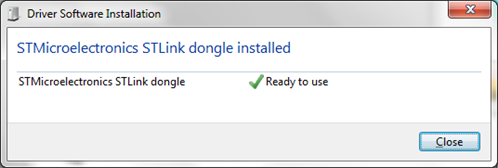
\includegraphics[width=0.6\textwidth]{stready}
\end{figure}
\par
Whilst the USB drivers are crucial for us, the actual ST-Link utility isn't necessary but it is very useful. If you really mess up the program running on the micro or incompletely flash a program to it, it will let you erase the memory on board your STM32 micro.
\\
Run the STM32 ST-Link Utility from wherever you installed it to and press the \textbf{\color{Purple} Connect to the Target} button 

\includegraphics[height=3ex]{conico}
. There should now be a flashing green and red LED on your board and the table in the program will be populated with memory addresses (from 0x0800000 onwards) and hexadecimal numbers. 
